\documentclass[12pt]{article}
%% arXiv paper template by Flip Tanedo
%% last updated: Dec 2016



%%%%%%%%%%%%%%%%%%%%%%%%%%%%%
%%%  THE USUAL PACKAGES  %%%%
%%%%%%%%%%%%%%%%%%%%%%%%%%%%%

\usepackage{amsmath}
\usepackage{amssymb}
\usepackage{amsfonts}
\usepackage{graphicx}
\usepackage{xcolor}
\usepackage{nopageno}
\usepackage{enumerate}
\usepackage{parskip}


\renewcommand{\thesection}{}
\renewcommand{\thesubsection}{\arabic{subsection}}

%%%%%%%%%%%%%%%%%%%%%%%%%%%%%%%%%%%%%%%%%%%%%%%
%%%  PAGE FORMATTING and (RE)NEW COMMANDS  %%%%
%%%%%%%%%%%%%%%%%%%%%%%%%%%%%%%%%%%%%%%%%%%%%%%

\usepackage[margin=2cm]{geometry}   % reasonable margins

\graphicspath{{figures/}}	        % set directory for figures

% for capitalized things
\newcommand{\acro}[1]{\textsc{\MakeLowercase{#1}}}    

\numberwithin{equation}{section}    % set equation numbering
\renewcommand{\tilde}{\widetilde}   % tilde over characters
\renewcommand{\vec}[1]{\mathbf{#1}} % vectors are boldface

\newcommand{\dbar}{d\mkern-6mu\mathchar'26}    % for d/2pi
\newcommand{\ket}[1]{\left|#1\right\rangle}    % <#1|
\newcommand{\bra}[1]{\left\langle#1\right|}    % |#1>
\newcommand{\Xmark}{\text{\sffamily X}}        % cross out

\let\olditemize\itemize
\renewcommand{\itemize}{
  \olditemize
  \setlength{\itemsep}{1pt}
  \setlength{\parskip}{0pt}
  \setlength{\parsep}{0pt}
}


% Commands for temporary comments
\newcommand{\comment}[2]{\textcolor{red}{[\textbf{#1} #2]}}
\newcommand{\flip}[1]{{\color{red} [\textbf{Flip}: {#1}]}}
\newcommand{\email}[1]{\texttt{\href{mailto:#1}{#1}}}

\newenvironment{institutions}[1][2em]{\begin{list}{}{\setlength\leftmargin{#1}\setlength\rightmargin{#1}}\item[]}{\end{list}}


\usepackage{fancyhdr}		% to put preprint number



% Commands for listings package
%\usepackage{listings}      % \begin{lstlisting}, for code
%
% \lstset{basicstyle=\ttfamily\footnotesize,breaklines=true}
%    sets style to small true-type



%%%%%%%%%%%%%%%%%%%
%%%  HYPERREF  %%%%
%%%%%%%%%%%%%%%%%%%

%% This package has to be at the end; can lead to conflicts
\usepackage{microtype}
\usepackage[
	colorlinks=true,
	citecolor=black,
	linkcolor=black,
	urlcolor=green!50!black,
	hypertexnames=false]{hyperref}





\begin{document}


\begin{center}

    {\Large \textsc{Short HW 3}:
    \textbf{Indices}}
    
\end{center}

\vskip .4cm

\noindent
\begin{tabular*}{\textwidth}{rl}
	\textsc{Course:}& Physics 165, \emph{Introduction to Particle Physics} (2018)
	\\
	\textsc{Instructor:}& Prof. Flip Tanedo (\email{flip.tanedo@ucr.edu})
	\\
	\textsc{Due by:}& \textbf{Thursday}, January 18
\end{tabular*}

\noindent
Note that this short assignment is due in class on Thursday. You have only \emph{two days} to do it. This should be quick, I recommend doing it right after class on Tuesday.

\subsection{The Yukawa interaction}

Consider the following toy theory of spin-1/2 particles interacting with a spin-0 particle. The theory has an SU(2) symmetry with doublet indices $a,b,c,\cdots \in \{1,2\}$ and triplet indices $A,B,\cdots \in \{1,2,3\}$. You have the following tensors:

\begin{itemize}
	\item {Lorentz metrics}: metric for vectors ($\eta^{\mu\nu}$, $\eta_{\mu\nu}$), metric for spinors ($\varepsilon^{\alpha\beta}$, $\varepsilon_{\alpha\beta}$, $\varepsilon^{\dot\alpha\dot\beta}$, $\varepsilon_{\dot\alpha\dot\beta}$)
	\item {Lorentz tensor}: $\sigma$-matrices ($\sigma^{\mu}_{\phantom\mu \alpha\dot\beta}$)
	\item SU(2) metrics: $\epsilon_{ab}$, $\epsilon^{ab}$, $\delta_{AB}$ (i.e.\ you can contract two upper $A$ indices)
	\item SU(2) tensors: $f^{abc}$, $T^{Aa}_{\phantom{Aa}b}$
	\item The identity: $\delta^a_b$, $\delta^\alpha_\beta$, etc.
	\item Momenta: $p^\mu$ of any particle going into the vertex
\end{itemize}

You have the following particles:
\begin{center}
	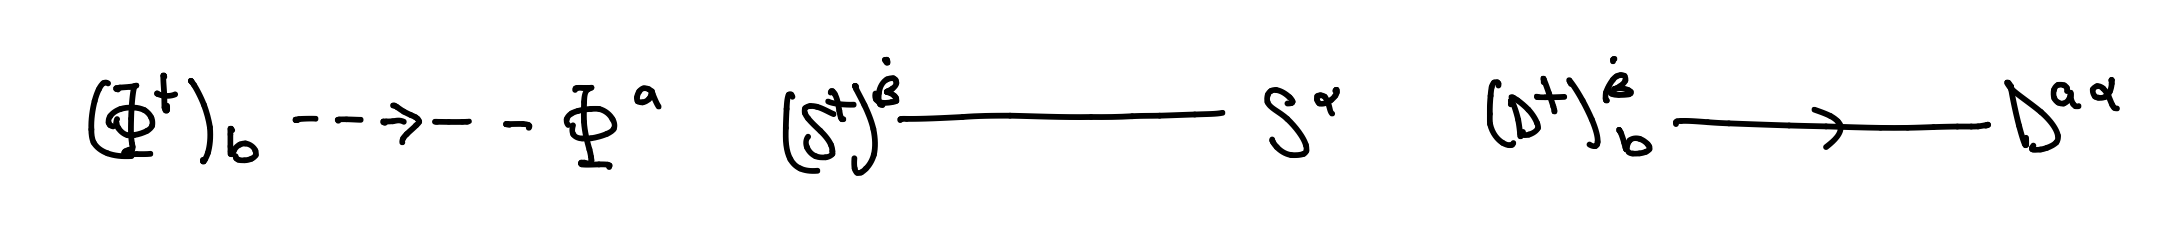
\includegraphics[width=.7\textwidth]{HW3a.png}
\end{center}
Here $\Phi^a$ is an SU(2) doublet, meaning it has two components. It has an anti-particle, $(\Phi^\dag)_b$. Observe that $\Phi$ is a Lorentz scalar: it doesn't have any spinor or vector index. The particle $S$ is a spin-1/2 particle that is an SU(2) singlet (``SU(2) scalar''), it has a spinor index but does not have any SU(2) indices. It has an antiparticle $(S^\dag)^{\dot \beta}$ The particle $D$ is an SU(2) doublet and a spin-1/2 particle with spinor indices. It has an anti-particle $(D^\dag)^{\dot \beta}_{\phantom\beta b}$.


Show that you can write down the following Feynman rules:
\begin{center}
	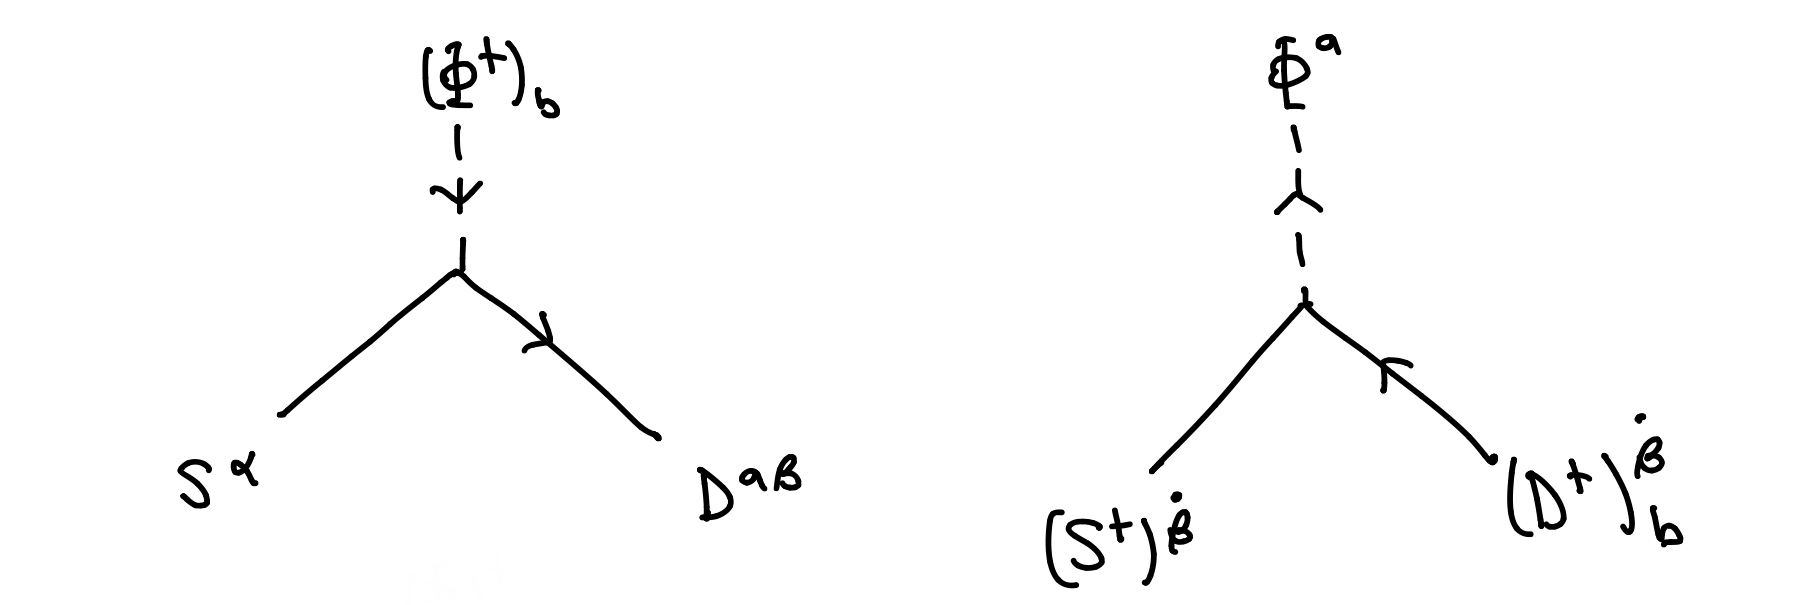
\includegraphics[width=.5\textwidth]{HW3aa.png}
\end{center}
That is, for each proposed Feynman rule, write down an invariant using the tensors above and the particles. For example,  your answer for the first diagram should look like:
\begin{align*}
	S^\alpha (\Phi^\dag)_b D^{a\beta} \left[\text{some combination of tensors}\right]^{b}_{\phantom{b}\alpha\beta a}
\end{align*}
\textsc{Remarks}: Don't confuse $a$ and $\alpha$. The $S$ has no arrow because it carries no charge.


\end{document}